\section{Problem 1}
\textit{Consider a street with infinite sides and a ground. For simplicity assume that both antennas are in the middle of the street. Apply a simple model using image theory with N reflections from the sides using a negative reflection coefficient.}\\

\textit{For positions along the street, find the:}

\textit{
\begin{pitemize}
\item field strength in dB without considering the antenna gains . What is the general trend (path loss) and fine structure (fading) vs range - and how does it change when different number of reflections are taken into account
\item infinite bandwidth impulse response- how does it vary with range and max number of reflections
\end{pitemize}
}

The problem sketch is found in \figref{fig:sketch_mm10}. 
\begin{figure}[!h]
  \centering
  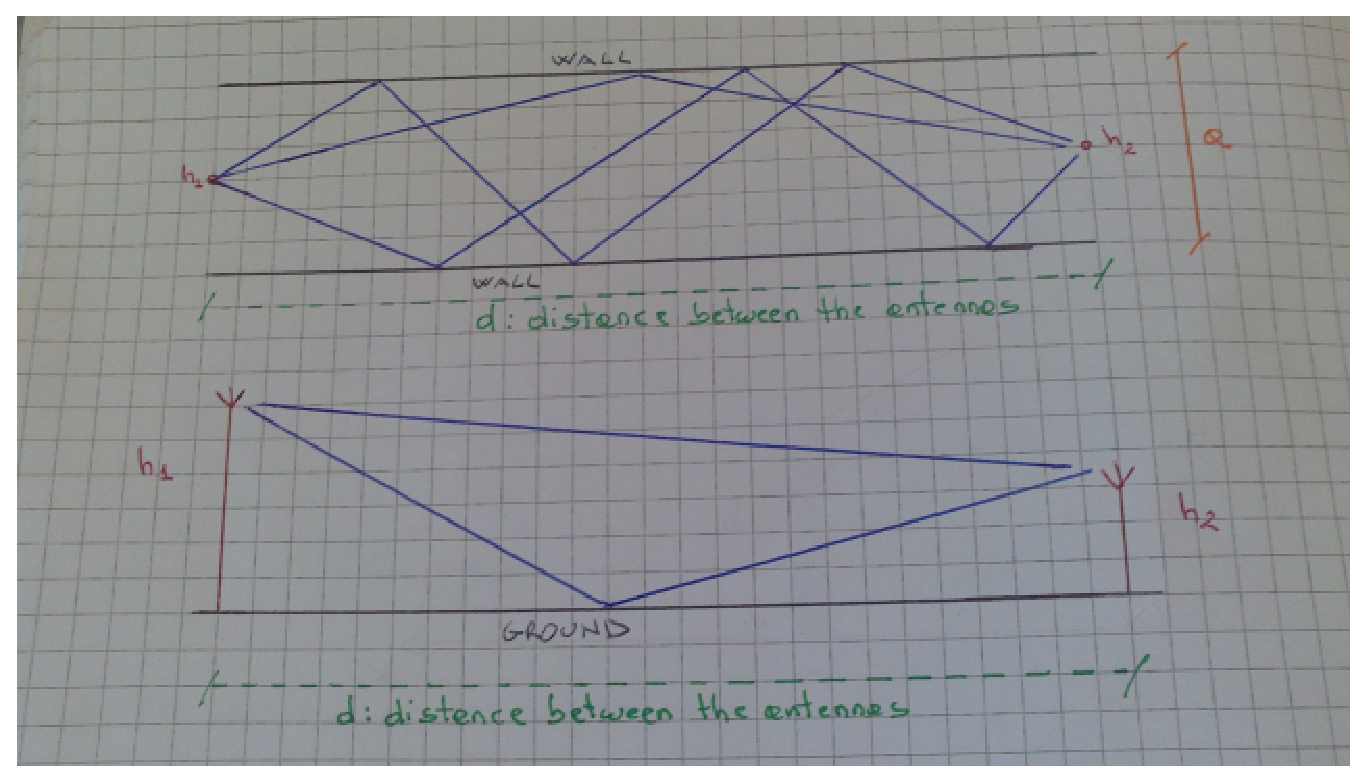
\includegraphics[width=12cm]{sketch_mm10.eps}
  \caption{Sketch for reflections on a street with infinite sides and a ground}
  \label{fig:sketch_mm10}
\end{figure}
In this scenario image theory is applied with N reflections using a negative reflection coefficient. Its negative value means that the reflected wave is shifted in phase by \SI{180}{\degree} ($\pi$). The antenna heights are denoted by $h_{1}$ and $h_{2}$ and $a$ represents the distance between the walls.

Using this scenario, the field strength is expressed in dB and the antenna gains are not considered. The path loss and field strength are represented as a function of distance in \figref{fig:field_pathloss}.
\begin{figure}[!h]
  \centering
  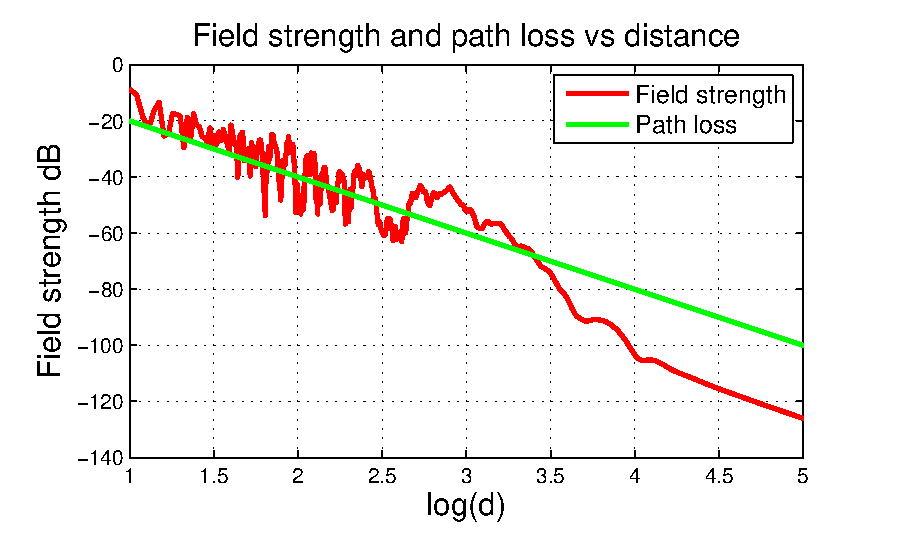
\includegraphics[width=12cm]{field_pathloss.eps}
  \caption{Sketch for reflections on a street with infinite sides and a ground}
  \label{fig:field_pathloss}
\end{figure}
This has been obtaint through the formulation below: 
\code{language=Matlab, caption = Field strength in dB, label=cl:Field strength in dB,linerange={28-40},firstnumber=1}{code/mm10/exercise_A_MM10.m} 
where N is the number of reflection,$ R_{w}$ is the reflection coefficient for the wall and $R_{g}$ is the reflection coefficient for the ground, Floss is the free space pathloss.

\textit{
\begin{pitemize}
\item infinite bandwidth impulse response- how does it vary with range and max number of reflections
\end{pitemize}
}

In this section we are going to build the impulse response in function of the delay for different distances: $dref_1$=100 and $dref_2$= 200. The delay is calculate 

\begin{figure}[!h]
  \centering
  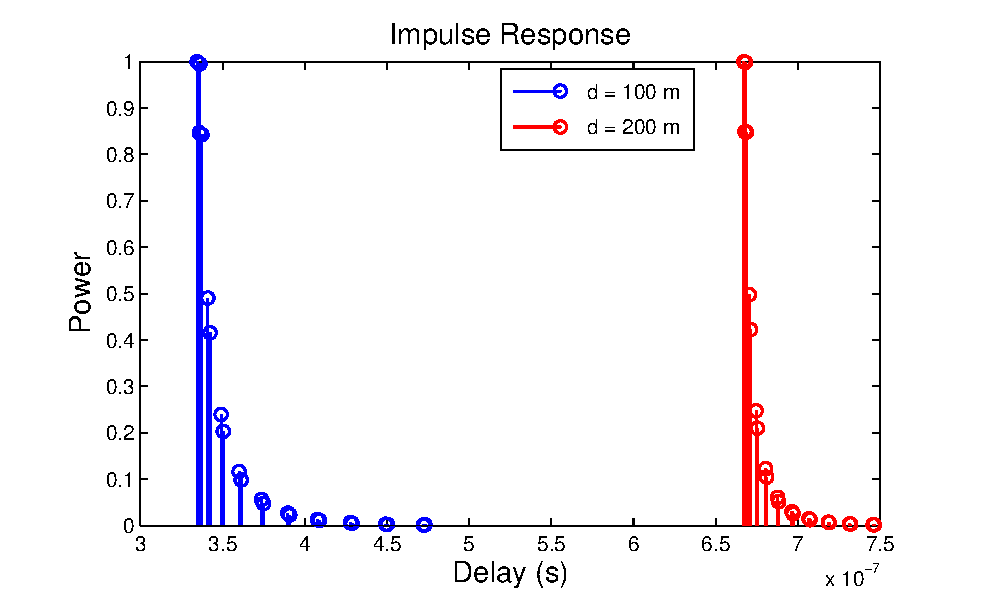
\includegraphics[width=18cm]{Impulse_Response.eps}
  \caption{Impulse response in function of the delay}
  \label{fig:field_pathloss}
\end{figure}

\begin{figure}[!h]
  \centering
  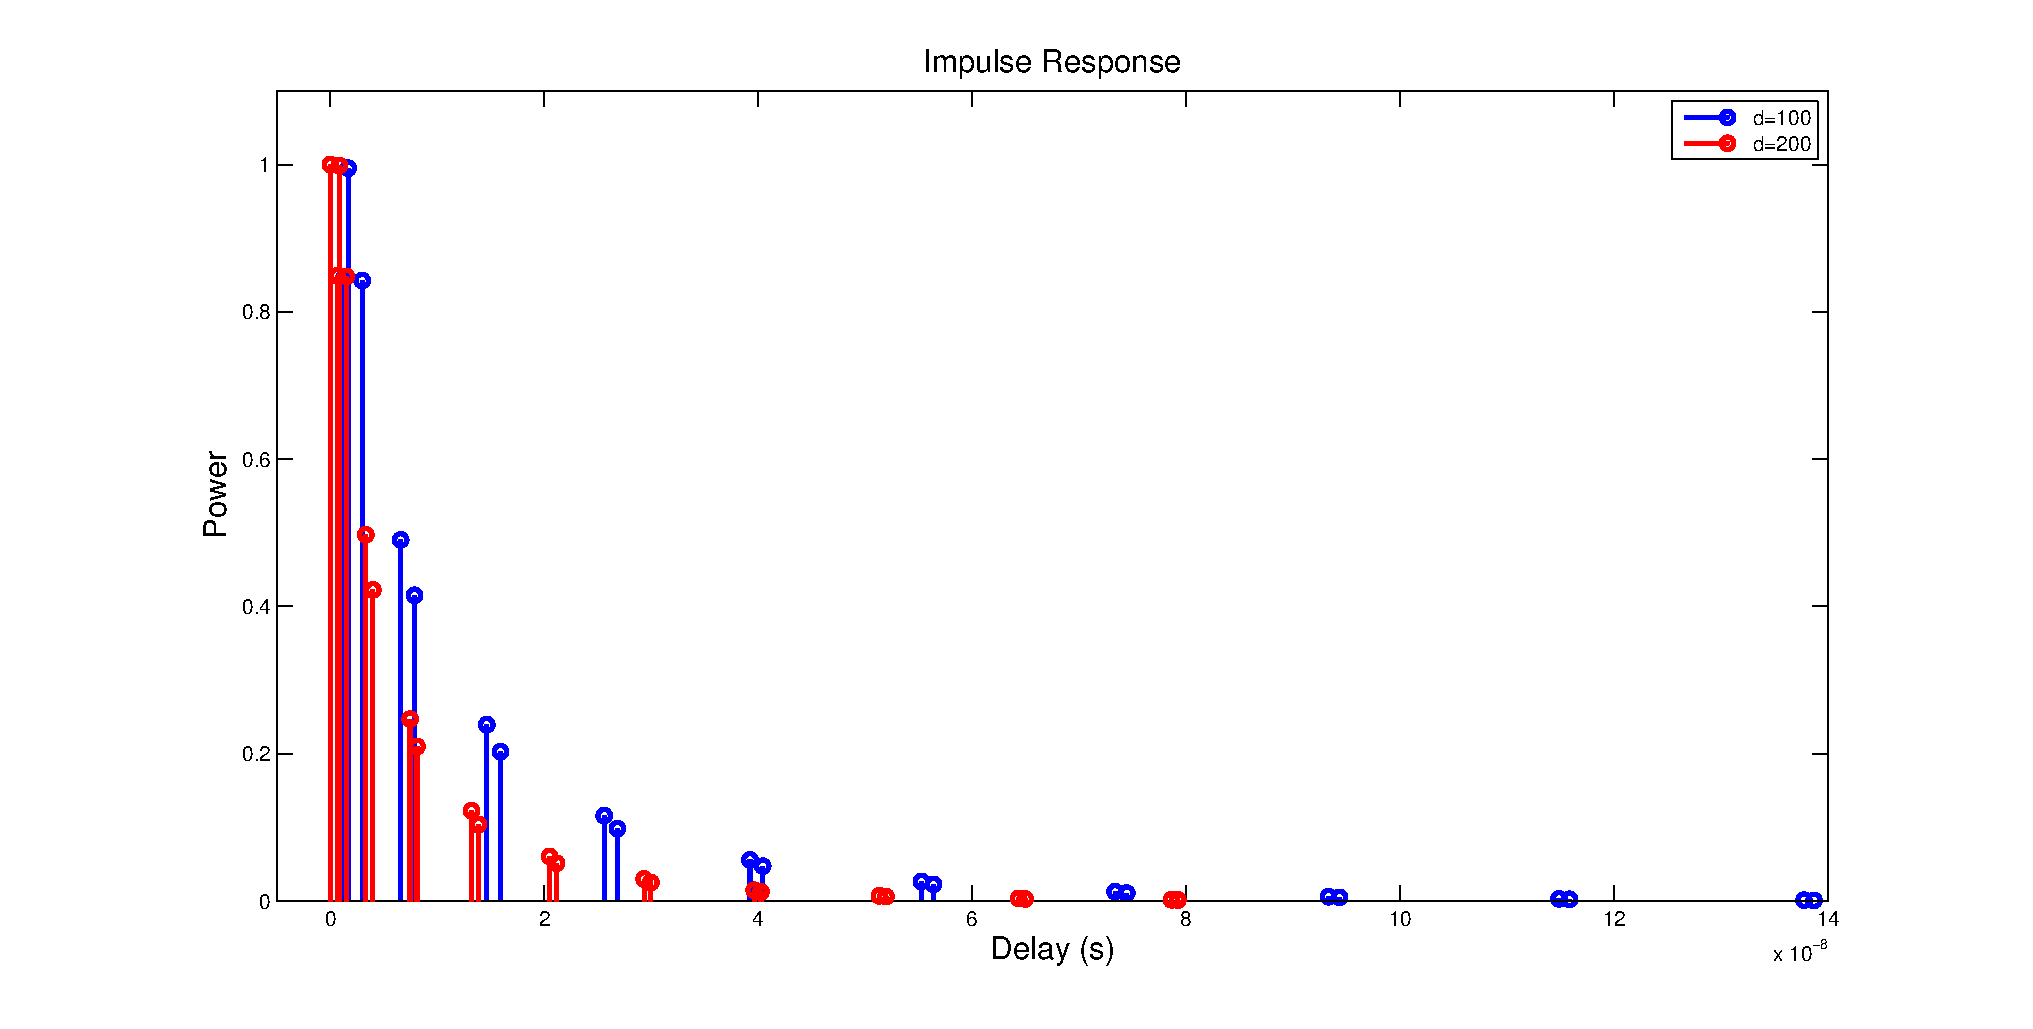
\includegraphics[width=18cm]{Impulse_Response_Delay_norm.eps}
  \caption{Impulse response in function of the delay with the first tap received}
  \label{fig:field_pathloss}
\end{figure}
